\section{Mathematical Expectation}

\subsection{Definition of Mathematical Expectation}

  For a discrete random variable $X$ taking values $x_{1},...,x_{n},$ the \emph{mathematical expectation} is defined as
  \begin{align}
   \label{eq:2.9.1}
   E(X)=\sum _{j=1}^{n} x_{j}P(X=x_{j})=:\sum xP(X=x),
  \end{align}
or equivalently
  \begin{align}
   \label{eq:2.9.2}
   E(X)=\sum _{j=1}^{n} x_{j}f(x_{j})=:\sum xf(x),
  \end{align}
  where $f(x)=P(X=x).$

 As a special case, when $f(x)\equiv \frac{1}{n},$ we obtain the \emph{arithmetic mean:}
 \begin{align}
  \label{eq:2.9.3}
  E(X)=\dfrac{\sum_{i=1}^{n}x_{i}}{n}.
 \end{align}

{}
\begin{ejemplo}
 Let $X$ be the number obtained when rolling a die. Then each face $x$ has the same probability
 \begin{align}
 f(x) = \frac{1}{6}
\end{align} of occurring.

Therefore,
$E(X)= (1)\left( \frac{1}{6} \right)+...+(6)\left( \frac{1}{6} \right) = \dfrac{1+...+6}{6} = 3.5$
\end{ejemplo}

{Countable Discrete Case}
 In the case where $X$ takes a countably infinite number of values $x_{1},x_{2},...,$ we define
 \begin{align}
  E(X)=\sum_{i=1}^{\infty}x_{i}f(x_{i}),
 \end{align}
provided that this \emph{series} converges absolutely.

% {}
% The above series must be understood as the limit
% $\lim_{n\to \infty} \sum_{i=1}^{n} x_{i}f(x_{i}).$
%
%
% 

{Continuous Case}
 For a continuous random variable $X$ having probability density function $f(x),$ the expectation of $X$ is defined as
 \begin{align}
  \label{eq:2.9.4}
  E(X)=\int_{-\infty}^{\infty}xf(x)dx
 \end{align}
provided that this \emph{integral} converges absolutely.

 The expectation of $X$ is often called the \emph{mean} of $X$ and is denoted by $\mu_{x},$ or simply $\mu,$ when the underlying random variable is understood from context.

 The mean or expectation of $X$ yields a single value representing the average of the values of $X,$ and for this reason we say that it is a \emph{measure of central tendency.}

 \begin{ejemplo}
  \label{exmp:2.9.1}
  Suppose a game is played with a single die assumed to be fair. In this game, a player wins \$20 if a $2$ turns up; \$40 with a $4$; \$30 with a $6$; and neither wins nor loses with any other face. Find the expected amount of money the player will win.
 \end{ejemplo}

\begin{solucion}
	Let $X$ be the player's winnings. The probability function is:
	\begin{align}
		f(x) = \begin{cases}
			\frac{1}{6} & x = 20 \\
			\frac{1}{6} & x = 40 \\
			\frac{1}{6} & x = 60 \\
			\frac{3}{6} & x = 0
		\end{cases}
	\end{align}
	
	The mathematical expectation is:
	\begin{align}
		\mu &= E(X) = \sum x \cdot f(x) \\
		&= 20 \cdot \frac{1}{6} + 40 \cdot \frac{1}{6} + 60 \cdot \frac{1}{6} + 0 \cdot \frac{3}{6} \\
		&= \frac{20 + 40 + 60}{6} = \frac{120}{6} = \$20
	\end{align}
	
	On average, the player wins \$20 per game.
\end{solucion}

 \begin{ejemplo}
  \label{exmp:2.9.2}
  The density function of a random variable $X$ is given by
  \begin{align}
   f(x)=
   \begin{cases}
    \frac{1}{2}x & 0<x<2 \\
    0 & \texttt{otherwise}
   \end{cases}
  \end{align}
Find the expected value of $X.$
 \end{ejemplo}

{}
\begin{align}
 \mu &= E(X)\\ & = \int_{-\infty}^{\infty} xf(x) dx \\
  &= \int_{0}^{2} x\left( \dfrac{1}{2}x \right) dx\\
  &= \evat{\frac{1}{6} \, x^{3}}{0}{2}\\
  &= \frac{1}{6}(2)^{3}-\frac{1}{6}(0)^{3} \\
  &= \frac{4}{3}
\end{align}

\subsection{Functions of Random Variables}

 Let $X$ be a discrete random variable with probability function $f(x).$ Then $Y=g(X)$ is a discrete random variable with probability function
 \begin{align}
  h(y)=P(g(X)=y)=\sum_{\set{x|g(x)=y}}g(x)f(x)
 \end{align}

 Therefore, in the discrete case:
 \begin{align}
 \label{eq:2.9.5}
  E\left( g(X) \right)=
  \sum_{x}g(x)f(x)
 \end{align}

 Similarly, in the continuous case:
 \begin{align}
  \label{eq:2.9.6}
  E\left( g(X) \right)=\int_{-\infty}^{\infty}
  g(x)f(x)dx.
 \end{align}

 \begin{ejemplo}
  \label{exmp:2.9.3}
  If $X$ is the random variable from Example \ref{exmp:2.9.2}, find $E\left( 3X^{2}-2X \right).$
 \end{ejemplo}

{}
In this case, $g(x)=3x^2-2x.$

Recall that
  \begin{align}
   f(x)=
   \begin{cases}
    \frac{1}{2}x & 0<x<2 \\
    0 & \texttt{otherwise}
   \end{cases}
  \end{align}

\begin{align}
 E(3X^2-2X) &= E(g(X)) \\
  &= \displaystyle \int_{-\infty}^{\infty} \left( 3x^2-2x \right)f(x)dx\\
  &= \displaystyle \int_{0}^{2}\left( 3x^2-2x \right)\left( \dfrac{1}{2}x \right)dx \\
  &= \displaystyle \int_{0}^{2} \frac{3}{2} \, x^{3} - x^{2} dx
 \\  &= \displaystyle \evat{\frac{3}{8} \, x^{4} - \frac{1}{3} \, x^{3}
}{0}{2}
\\  &= \displaystyle
\frac{10}{3}
\end{align}

\subsection{Some Theorems on Mathematical Expectation}
{Linearity}
 \begin{teorema}
  \label{thm:2.9.1}
  If $c,d$ are constants and $X,Y$ are random variables, then
  \begin{align}
   \label{eq:2.9.7}
   E\left( cX+dY \right)=
   cE\left( X \right)+dE\left( Y \right)
  \end{align}
 \end{teorema}

{Expectation and Independence}
 \begin{teorema}
  \label{thm:2.9.2} If $X,Y$ are \emph{independent random variables}, then
  \begin{align}
   \label{eq:2.9.8}
   E\left( XY \right)=E(X)E(Y)
  \end{align}
 \end{teorema}

\subsection{Variance and Standard Deviation}

 We have already seen that the mathematical expectation of a random variable $X$ is a measure of central tendency that generalizes the \emph{arithmetic mean $\mu$.}
 
\begin{observacion}
 For this reason, from now on we define
 \begin{align}
  \mu=\mu_{X}=E(X).
 \end{align}
\end{observacion}

 Another quantity of great importance is the \emph{variance}, which is defined as
 \begin{align}
  \label{eq:2.9.9}
  \s_{X}^{2}=\Var(X)=E\left( \left( X-\mu_{X} \right)^{2} \right)
 \end{align}

 The \emph{standard deviation} is defined as
 \begin{align}
  \label{eq:2.9.10}
  \s_{X} = \sqrt{\Var{X}}
 \end{align}

 \begin{observacion}
  If the random variable $X$ is understood from context, we will omit the corresponding subscript; that is,
  \begin{align}
   \mu=\mu_{X}, \; \s=\s_{X}, \; \s^{2}=\s_{X}^{2}.
  \end{align}
 \end{observacion}

 If $X$ is a discrete random variable, the variance is given by
 \begin{align}
  \label{eq:2.9.11}
  \s^{2}=E\left( \left( X-\mu \right)^{2} \right)=\sum\left( x-\mu \right)^{2}f(x),
 \end{align}
 provided that this sum converges.

If all probabilities are equal and the random variable $X$ takes finite values, we have
\begin{align}
\label{eq:2.9.12}
 \s^{2}=\dfrac{\left( x_{1}-\mu \right)^{2}+...+\left( x_{n}-\mu \right)^{2} }{n}
\end{align}

{}
\begin{ejemplo}
 As seen previously, if $X$ is the face obtained when rolling a die, then $\mu_{X}=3.5$.

The variance of $X$ is
\begin{align}
 \s^{2}
 &= \displaystyle \dfrac{(1-3.5)^2+...+(6-3.5)^2}{6}
 \\  &= \displaystyle \frac{17.5}{6}
 \\  &\approx \displaystyle 2.916
\end{align}
\end{ejemplo}

 If $X$ is a continuous random variable with density function $f(x),$ then the variance is given by
 \begin{align}
  \label{eq:2.9.13}
  \s^{2}=E\left( (X-\mu)^{2} \right)=
  \int_{-\infty}^{\infty}\left( x-\mu \right)^{2}f(x)dx
 \end{align}
provided the integral converges.

 Both the variance and standard deviation are \emph{measures of dispersion.}
 \begin{figure}
 \centering
 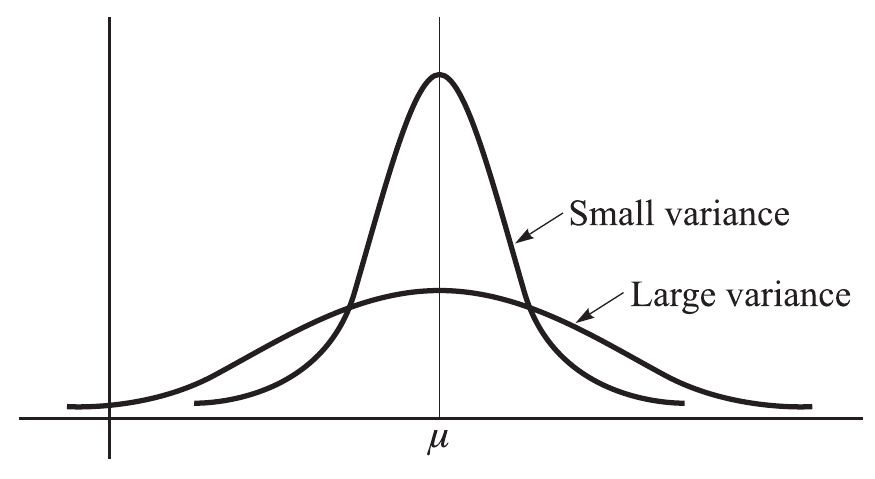
\includegraphics[height=5cm,keepaspectratio=true]{./pe/pands0301.png}
 % pands0301.png: 0x0 pixel, 300dpi, 0.00x0.00 cm, bb=
 \label{fig:2.9.1}
\end{figure}

 \begin{ejemplo}
  \label{exmp:2.9.4}
  Find the variance and standard deviation of the random variable from Example \ref{exmp:2.9.2}.
 \end{ejemplo}

{}
Recall that this random variable $X$ has probability density
  \begin{align}
   f(x)=
   \begin{cases}
    \frac{1}{2}x & 0<x<2 \\
    0 & \texttt{otherwise}
   \end{cases}
  \end{align}

{}
\begin{align}
 \sigma^2 = Var(X) &= \displaystyle \int_{0}^{2}(x-\frac{4}{3})^2f(x) dx
 \\  &= \displaystyle \int_{0}^{2} \frac{1}{2} \, {\left(x - \frac{4}{3}\right)}^{2} x dx
 \\  &= \displaystyle
 \evat{\frac{1}{8} \, x^{4} - \frac{4}{9} \, x^{3} + \frac{4}{9} \, x^{2}}{0}{2}
 \\  &= \displaystyle \frac{2}{9}
\\  &\approx \displaystyle 0.\bar{2}
\end{align}

{Some Theorems on Variance}
\begin{align}
 \label{eq:2.9.14}
 \s^{2}=E\left( X^{2} \right)-\mu^{2} \\ 
 \label{eq:2.9.15}
 \Var\left( cX \right)=c^{2}\Var\left( X \right)\\ 
 \label{thm:2.9.3}
 \s^{2}=\min_{a}\set{E\left( \left( X-a \right)^{2} \right)}
\end{align}

If $X,Y$ are independent:
\begin{align}
 \label{eq:2.9.16}
 \Var(X\pm Y)=\Var(X)+\Var(Y)
\end{align}

{Standardized Random Variables}
 Let $X$ be a random variable with mean $\mu$ and standard deviation $\s>0.$ We say that the associated \emph{standardized random variable} is given by
 \begin{align}
  \label{eq:2.9.17}
  X^{*}=\dfrac{X-\mu}{\s}.
 \end{align}

\begin{align}
 \label{eq:2.9.18}
 E\left( X^{*} \right)=0, \; \Var(X^{*})=1.
\end{align}

\subsection{Covariance and Correlation}

The results given previously for a single random variable can be extended to two variables.

{}

\[
 \label{eq:2.9.19}
 \begin{split}
  \mu_{X}=E(X)=\int_{-\infty}^{\infty}\int_{-\infty}^{\infty} xf(x,y)dxdy\\ 
  \mu_{Y}=E(Y)=\int_{-\infty}^{\infty}\int_{-\infty}^{\infty}
  yf(x,y)dxdy
 \end{split}
\]

\[
 \label{eq:2.9.20}
 \begin{split}
  \s^{2}_{X}=E\left( (X-\mu_{X})^{2} \right)=\int_{-\infty}^{\infty}\int_{-\infty}^{\infty} (x-\mu_{X})^2f(x,y)dxdy\\ 
  \s^{2}_{Y}=E\left( (Y-\mu_{Y})^{2} \right)=\int_{-\infty}^{\infty}\int_{-\infty}^{\infty} (y-\mu_{Y})^2f(x,y)dxdy
 \end{split}
\]

{Covariance}
 \begin{align}
 \label{eq:2.9.21}
  \s_{XY}=\cov(X,Y)=E\left( (X-\mu_{X})(Y-\mu_{Y}) \right)
 \end{align}

 \begin{align}
  \label{eq:2.9.22}
  \s_{XY}=\int_{-\infty}^{\infty}
  \int_{-\infty}^{\infty}
  (x-\mu_{X})(y-\mu_{Y})f(x,y)dxdy
 \end{align}

{Discrete Case}

 \[
  \begin{split}
   \mu_{X}=\sum_{x}\sum_{y}xf(x,y) \\
  \mu_{Y}=\sum_{x}\sum_{y}yf(x,y)
  \end{split}
 \]

 \begin{align}
  \label{eq:2.9.23}
  \s_{XY}=\sum_{x}\sum_{y}(x-\mu_{X})(y-\mu_{Y})f(x,y)
 \end{align}

 \begin{align}
  \label{eq:2.9.24}
  \s_{XY}=E(XY)-E(X)E(Y)=E(XY)-\mu_{X}\mu_{Y}
 \end{align}

 If $X,Y$ are independent, then
 \begin{align}
  \label{eq:2.9.24a}
  \s_{XY}=\cov(X,Y)=0
 \end{align}

 \begin{align}
  \label{eq:2.9.25}
  \Var(X\pm Y)=\Var(X)\pm2\cov(X,Y)+\Var(Y).
 \end{align}

 Equivalently,
 \begin{align}
  \label{eq:2.9.26}
  \s_{X\pm Y}^{2}=\s_{X}^{2} \pm 2\s_{XY} +\s_{Y}^{2}
 \end{align}

{Pearson Correlation Coefficient}
 \begin{align}
  \label{eq:2.9.27}
  \rho = \dfrac{\s_{XY}}{\s_{X}\s_{Y}}
 \end{align}

 \begin{teorema}
  \begin{align}
   \label{eq:2.9.28}
   \abs{\s_{XY}}\leq \s_{X}\s_{Y}
  \end{align}

 \begin{align}
  \abs{\rho}\leq 1.
 \end{align}
 \end{teorema}

{Properties of Correlation}

\begin{enumerate}
\item $-1 \leq \rho \leq 1$ 
 \item $\rho \approx 0$: \emph{Weak correlation}, virtually no linear correlation exists. 
 \item $\abs{\rho} \approx 1$: \emph{Strong correlation}, the correlation is almost perfectly described by an affine function $y=mx+b$. 
 \item $\rho > 0$: \emph{Positive correlation}, as one increases, the other increases as well. 
 \item $\rho < 0$: \emph{Negative correlation}, as one increases, the other decreases.
\end{enumerate}

 \begin{ejemplo}
  \label{exmp:2.9.5}
  \emph{Let $X,Y$ be discrete random variables} with joint probability density
  \begin{align}f(x,y)=
   \begin{cases}
    \dfrac{2x+y}{42} & 0\leq x \leq 2,\; 0\leq y \leq 3 \\
    0 & \texttt{otherwise}.
   \end{cases}
  \end{align}
 \end{ejemplo}
 
Find the following statistics:
\begin{multicols}{3}
 \begin{enumerate}
 \item $\mu_X = E(X)$ %
 \item $\mu_Y = E(Y)$ %
 \item $ E(XY)$ %
 \item $E(X^2)$ %
 \item $E(Y^2)$ %
 \item $\s^2_X = \Var(X)$ %
 \item $\s_{X}$
 \item $\s^2_Y = \Var(Y)$ %
 \item $\s_{Y}$
 \item $\s_{XY} =\cov(X,Y)$ %
 \item $\rho$
\end{enumerate}
\end{multicols}

 \begin{ejemplo}
  \label{exmp:2.9.6}
  \emph{Let $X,Y$ be continuous random variables} with joint probability density
  \begin{align}f(x,y)=
   \begin{cases}
    \frac{1}{210}(2x+y) & 2 < x < 6,\; 0<y<5 \\
    0 & \texttt{otherwise}.
   \end{cases}
  \end{align}
 \end{ejemplo}

Find the following statistics:
\begin{multicols}{3}
 \begin{enumerate}
 \item $\mu_X = E(X)$ %
 \item $\mu_Y = E(Y)$ %
 \item $ E(XY)$ %
 \item $E(X^2)$ %
 \item $E(Y^2)$ %
 \item $\s^2_X = \Var(X)$ %
 \item $\s_{X}$
 \item $\s^2_Y = \Var(Y)$ %
 \item $\s_{Y}$
 \item $\s_{XY} =\cov(X,Y)$ %
 \item $\rho$
\end{enumerate}
\end{multicols}
